\documentclass{chi-ext}
% Please be sure that you have the dependencies (i.e., additional LaTeX packages) to compile this example.
% See http://personales.upv.es/luileito/chiext/

%% EXAMPLE BEGIN -- HOW TO OVERRIDE THE DEFAULT COPYRIGHT STRIP -- (July 22, 2013 - Paul Baumann)
% \copyrightinfo{Permission to make digital or hard copies of all or part of this work for personal or classroom use is granted without fee provided that copies are not made or distributed for profit or commercial advantage and that copies bear this notice and the full citation on the first page. Copyrights for components of this work owned by others than ACM must be honored. Abstracting with credit is permitted. To copy otherwise, or republish, to post on servers or to redistribute to lists, requires prior specific permission and/or a fee. Request permissions from permissions@acm.org. \\
% {\emph{CHI'14}}, April 26--May 1, 2014, Toronto, Canada. \\
% Copyright \copyright~2014 ACM ISBN/14/04...\$15.00. \\
% DOI string from ACM form confirmation}
%% EXAMPLE END -- HOW TO OVERRIDE THE DEFAULT COPYRIGHT STRIP -- (July 22, 2013 - Paul Baumann)

\title{CCRec:Content of Publications and Collaboration Network Combined Academic Collaborators Recommendation}



\numberofauthors{6}
% Notice how author names are alternately typesetted to appear ordered in 2-column format;
% i.e., the first 4 autors on the first column and the other 4 auhors on the second column.
% Actually, it's up to you to strictly adhere to this author notation.
\author{
  \alignauthor{
  	\textbf{First Author}\\
  	\affaddr{AuthorCo, Inc.}\\
  	\affaddr{123 Author Ave.}\\
  	\affaddr{Authortown, PA 54321 USA}\\
  	\email{author1@anotherco.com}
  }\alignauthor{
  	\textbf{Fourth Author}\\
  	\affaddr{AuthorCo, Inc.}\\
  	\affaddr{123 Author Ave.}\\
  	\affaddr{Authortown, PA 54321 USA}\\
  	\email{author5@anotherco.com}
  }
  \vfil
  \alignauthor{
  	\textbf{Second Author}\\
  	\affaddr{AuthorCo, Inc.}\\
  	\affaddr{123 Author Ave.}\\
  	\affaddr{Authortown, PA 54321 USA}\\
  	\email{author2@anotherco.com}
  }\alignauthor{
  	\textbf{Fifth Author}\\
  	\affaddr{AuthorCo, Inc.}\\
  	\affaddr{123 Author Ave.}\\
  	\affaddr{Authortown, PA 54321 USA}\\
  	\email{author6@anotherco.com}
  }
  \vfil
  \alignauthor{
  	\textbf{Third Author}\\
  	\affaddr{AuthorCo, Inc.}\\
  	\affaddr{123 Author Ave.}\\
  	\affaddr{Authortown, PA 54321 USA}\\
  	\email{author3@anotherco.com}
  }\alignauthor{
  	\textbf{Sixth Author}\\
  	\affaddr{AuthorCo, Inc.}\\
  	\affaddr{123 Author Ave.}\\
  	\affaddr{Authortown, PA 54321 USA}\\
  	\email{author7@anotherco.com}
  }
}

% Paper metadata (use plain text, for PDF inclusion and later re-using, if desired)
\def\plaintitle{CHI LaTeX Extended Abstracts Template}
\def\plainauthor{Luis A. Leiva}
\def\plainkeywords{Guides, instructions, author's kit, conference publications}
\def\plaingeneralterms{Documentation, Standardization}

\hypersetup{
  % Your metadata go here
  pdftitle={\plaintitle},
  pdfauthor={\plainauthor},
  pdfkeywords={\plainkeywords},
  pdfsubject={\plaingeneralterms},
  % Quick access to color overriding:
  %citecolor=black,
  %linkcolor=black,
  %menucolor=black,
  %urlcolor=black,
}

\usepackage{graphicx}   % for EPS use the graphics package instead
\usepackage{balance}    % useful for balancing the last columns
\usepackage{bibspacing} % save vertical space in references
\usepackage{subfigure}
\usepackage{epstopdf}


\begin{document}

\maketitle

\begin{abstract}
With the academic research filed expanding, the problem of finding proper potential collaborators is really cumbersome. In this paper, we proposed a content of publications and collaboration network combined academic collaborators recommendation model (CCRec). Compared to traditional approaches, CCRec is more effective because it recommends collaborators combining the content of publications and collaboration network in different topics. Experiments based on DBLP data sets show that CCRec significantly outperforms traditional approaches, with the topic drift problem well solved.
\end{abstract}

\keywords{\plainkeywords}
\textcolor{red}{Mandatory section to be included in your final version.}

\category{H.5.m}{Information interfaces and presentation (e.g., HCI)}{Miscellaneous}.
%See \cite{ACMCCS}
See: \url{http://www.acm.org/about/class/1998/}
for help using the ACM Classification system.
\textcolor{red}{Mandatory section to be included in your final version.}

%\terms{\plaingeneralterms}
%\textcolor{red}{Optional section to be included in your final version.}


% =============================================================================
\section{Introduction}
% =============================================================================
Collaboration network is one kind of academic social networks formed by scholars and their collaborations. In the academic field, recommending collaborators to scholars or groups may help scholars build more collaborations and more prolific.

Studies show that they often recommend academic collaborators by exploiting the collaborations network and the profiles of scholars such as affiliation. However, the fact is always ignored that collaborations among scholars largely depend on the research field reflected from their publications. Thus it may have a superior performance to combine the content of publications and collaboration network to compare the similarity of scholars.

This paper proposed a content of publications and collaboration network combined academic collaborators recommendation model (CCRec). CCRec firstly uses the topic clustering (sensitive) to partition the words from all the publications titles into multiple domains. Then, CCRec computes the degree of interest (DoI) and the strength of influence (SoI) pertaining to each domain for each scholar. Finally, DoI and SoI combine to form the feature vector for each scholar and comparing the similarity of feature vector can get the recommending list.


% =============================================================================
\section{PROPOSED SCHEMA}
% =============================================================================
The CCRec is inspired by the truth that scholars usually desire to co-operate with people who have high similarity with them.
As mentioned above, scholars often behave differently across multiple domains of interest, which can denote scholars' academic features. In this work, TSCRec model contains a simple way to obtain these domains by a topic-clustering method. We define the DoI (degree of interest) and SoI (strength of influence) of scholars on different domains. Further more, we conduct vectors for every scholars based on these two metrics to measure the scholars academic feature.

%proposed a content based method to measure the "attention-degree" of scholars on different domains by parsing papers' title, and a graph based method to measure the %"influence-strength" by analysis the coauthor networks. Additionally, we merge the two metrics into "membership-degree" to measure the scholars academic interest feature. Finally, %we make a TopN recommendation based on the similarity of scholars' membership-degree vectors.

Fig. 1 depicts the four components of TSCRec: \textit{topic clustering and scholar partition}, \textit{Topic-sensitive random walk}, \textit{vector similarity calculation and TopN recommendation}. Topic clustering and scholar partition provide the distribution of scholars' interest in various domains and the DoIs of every scholar. Topic-sensitive random walk calculate scholars' influence in various domains and the SoIs of every scholar. Finally, The last component provide a TopN recommendation by the vectors similarity.

\begin{figure}
\centering
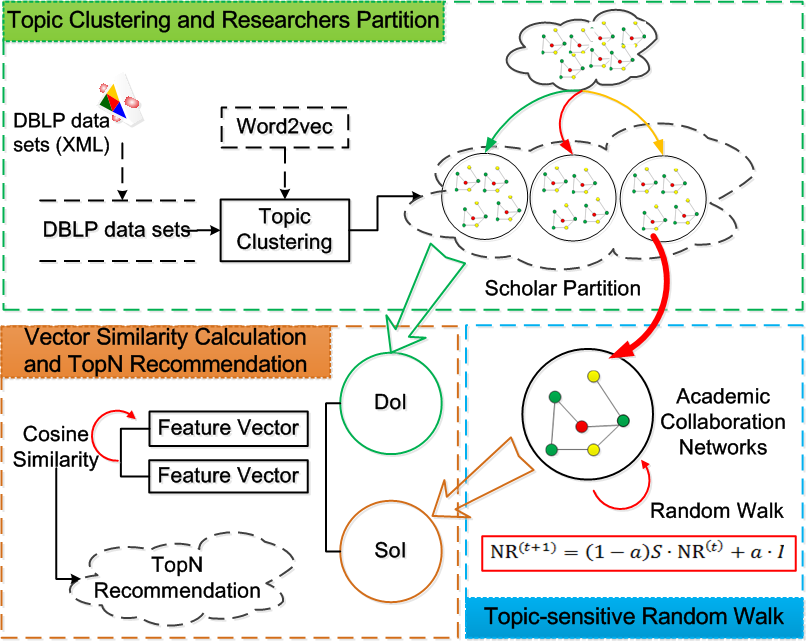
\includegraphics [width=3.4in]{Fig1.png}
\caption{The architecture diagram of TSCRec model}
\end{figure}

\subsection{Topic Clustering and Scholar Partition}
% -----------------------------------------------------------------------------
In TSCRec, topic clustering and scholar partition conducted various domains and map all scholars to these domains. Initially, TSCRec extract and parser key words from titles of all the papers in academic area and filter out some unworthy grammatical particle, e.g. "of", "the", "and". As a text corpus, these set of preprocessed key words are rich in a variety of academic topics. The word2vec, a famous tool of NLP (Natural Language Processing), is utilized to cluster the key words into different topics which can denote various academic domains. Afterwards, TSCRec extract the key words from titles of scholars' papers, and partition these scholars into different domains by mapping every authors' key words into relevant topics obtained above. Assuming that, there are some keywords of one scholar belongs to a topic, we will partition this scholar into this topic. What we can come up with is that, one scholar can appear in different domains for its diversity of interest which can exactly represent its distribution of scholars. In general, there are also a great many scholars in each domains.

\subsection{Feature Vector Calculation}
% -----------------------------------------------------------------------------
To measure the distribution of scholars' interest, we proposed DoI to define the scholar's proportion of interest in one domains:
\begin{equation}
DoI_{s,d}=\frac{N_{d}}{\sum_{k=1}^{n} N_{k}}
\end{equation}
It is a content-based method by utilizing the  information on the titles of scholars publications. Where $N_{d}$ is the number of key words of scholar $s$ in domains $d$.

We proposed SoI to define the scholar's strength of influence in one domains, which is measured by a random walk method based on co-authorship networks.
\begin{equation}
R_{d}^{(t+1)}=\alpha \mathbf{S}R_{d}^{(t)}+(1-\alpha)q
\end{equation}
It is a graph-based method by utilizing the information of co-authorship networks. Where $R_{d}$ represent the rank score vector of all scholars in domain $d$, $q$ is the initial vector of $R$, $\alpha$ denotes the damping coefficient. Random walk is a iterative process. After limited iterations, the vector $R$ will be convergent. We can get $SoI_{s}=R_{d,s}$.

To be more accurate, We define feature vector $F$ by combining $DoI$ and $SoI$, which measure the academic feature of scholar on various domains.

\begin{equation}
F_{s,d}=DoI_{s}*SoI_{s}
\end{equation}

\subsection{Collaborator Recommendation by Feature Vector Similarity}
% -----------------------------------------------------------------------------
In C2Rec, The academic feature of scholars is measured by the feature vector $F$. We use a \emph{cosine similarity} method to computing the similarity of these feature vectors, and further denoting the similarity between scholars.
\begin{equation}
SimCos(s_{1},s_{2})=\frac{\sum_{i=1}^{n}(F_{s_{1},i}*F_{s_{2},i})}{\sqrt{\sum_{i=1}^{n}F_{s_{1},i}^2}*\sqrt{\sum_{i=1}^{n}F_{s_{2},i}^2}}
\end{equation}

Finally, C2Rec recommend to scholars those potential collaborators who have high similarity with them, and provide a TopN collaborators recommendation list. 
% =============================================================================
\section{Evaluation and Analysis}
% =============================================================================
\begin{figure*}
\centering
\subfigure[Precision]{
\label{fig:2-a}
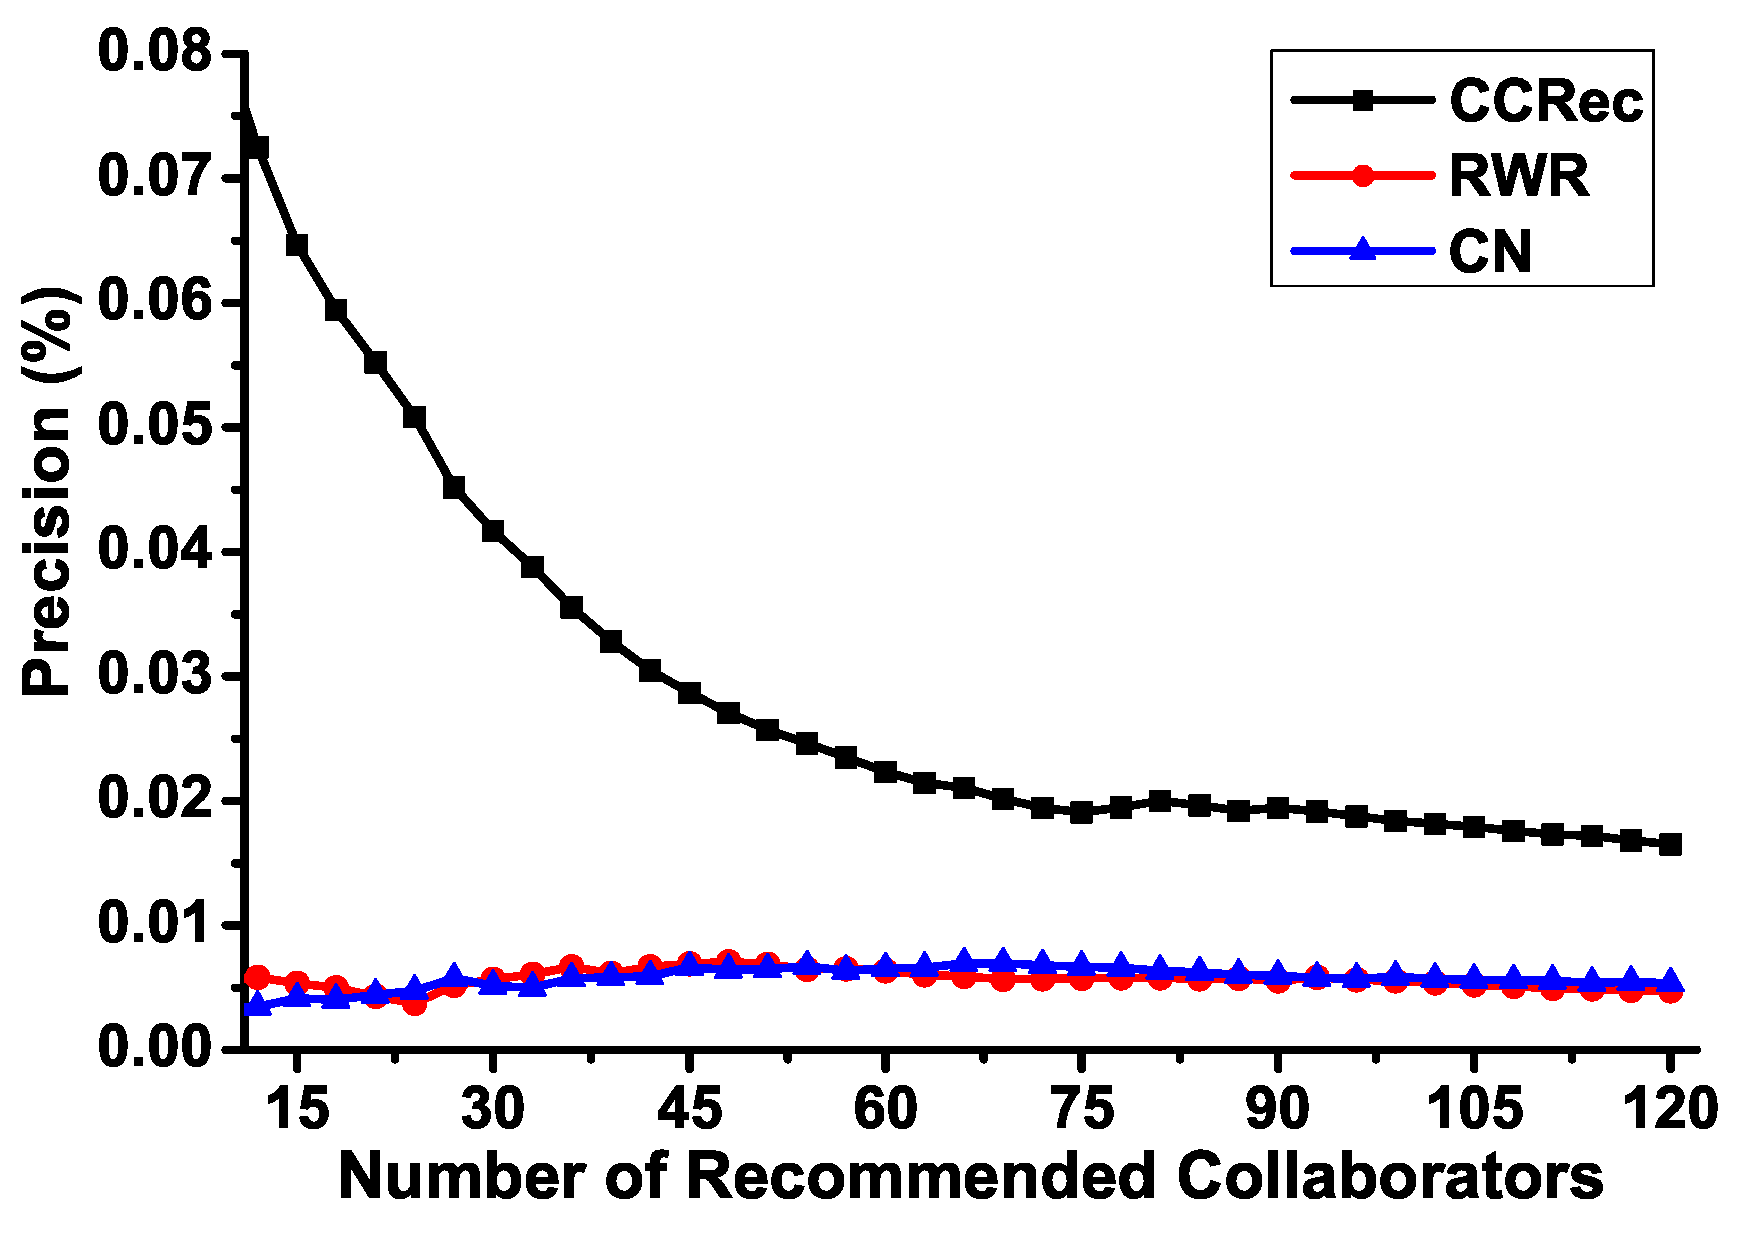
\includegraphics[width=0.32\textwidth]{Fig2-a.eps}}
\subfigure[Recall Rate]{
\label{fig:2-b}
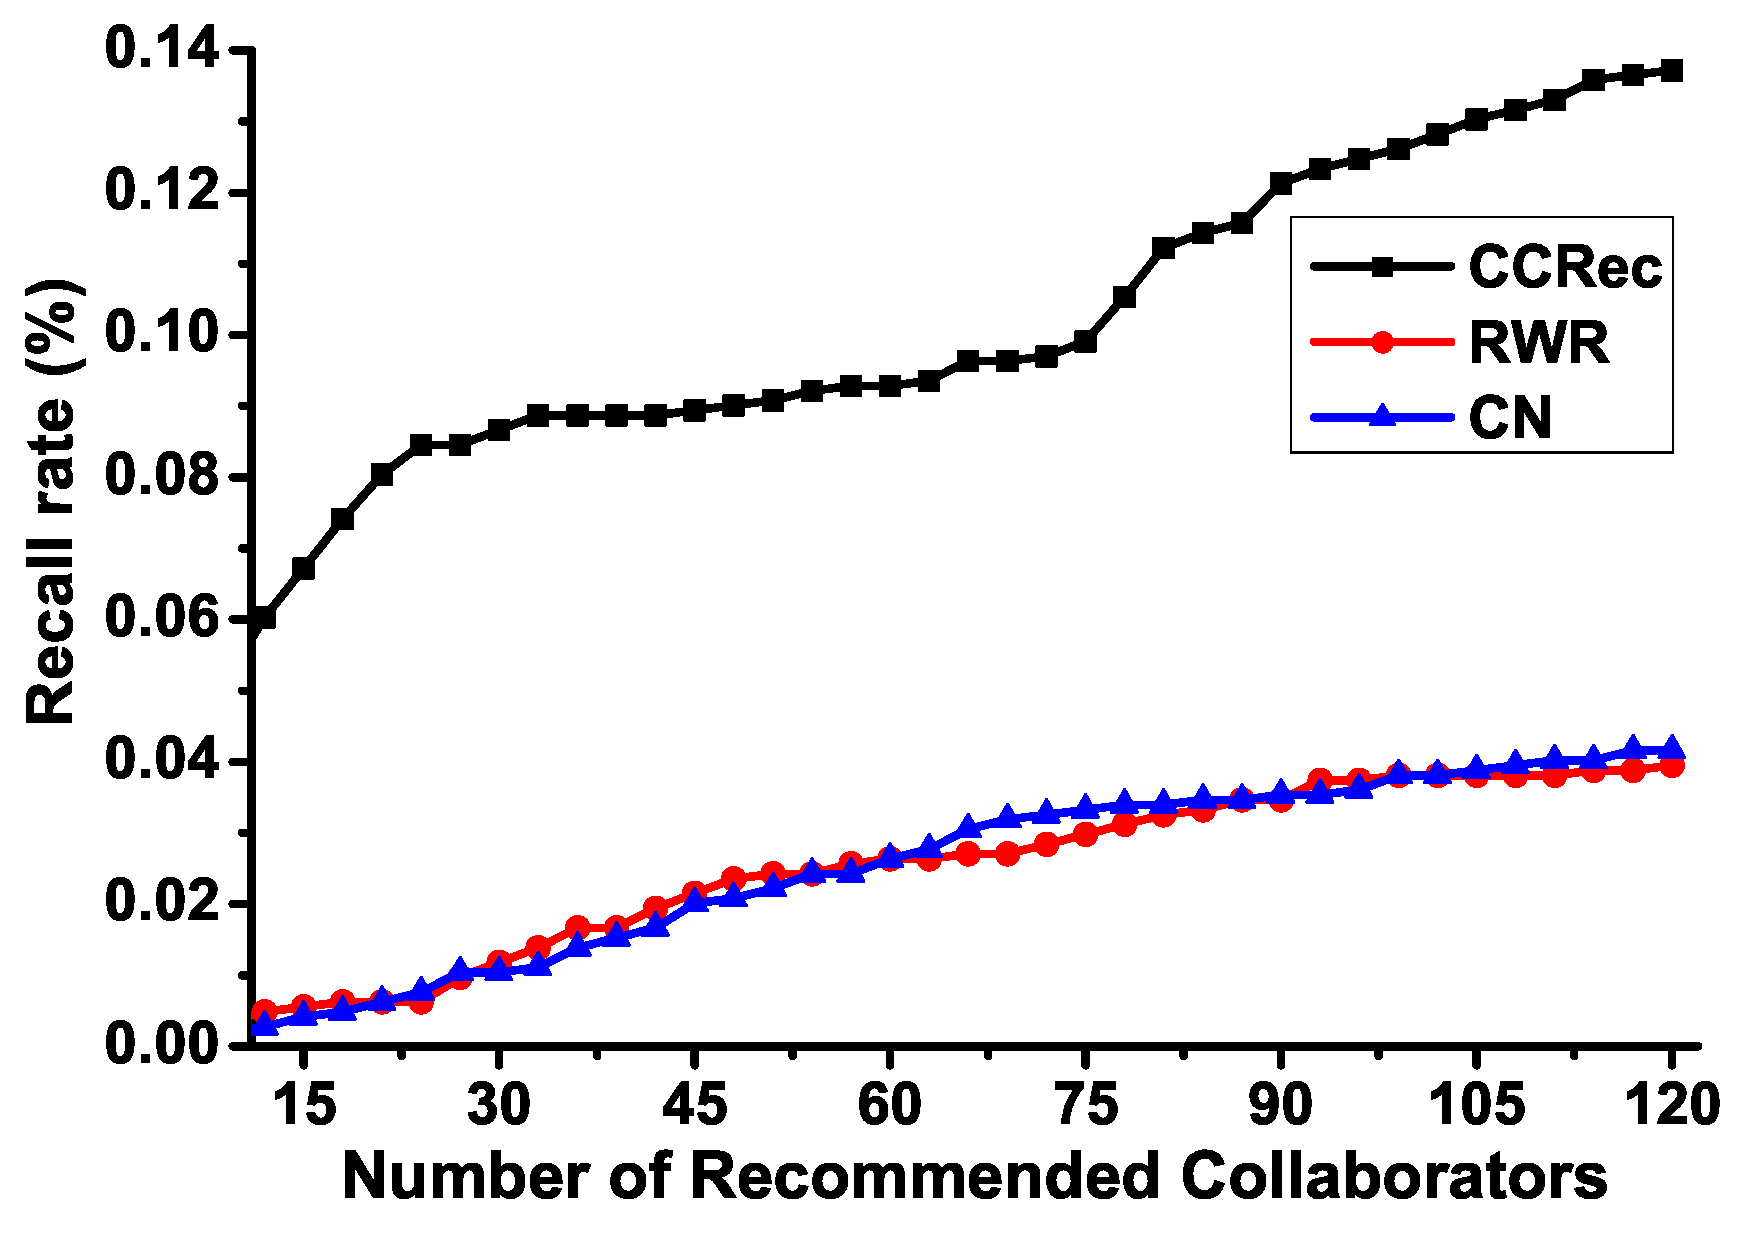
\includegraphics[width=0.32\textwidth]{Fig2-b.eps}}
\subfigure[Coverage Rate]{
\label{fig:2-c}
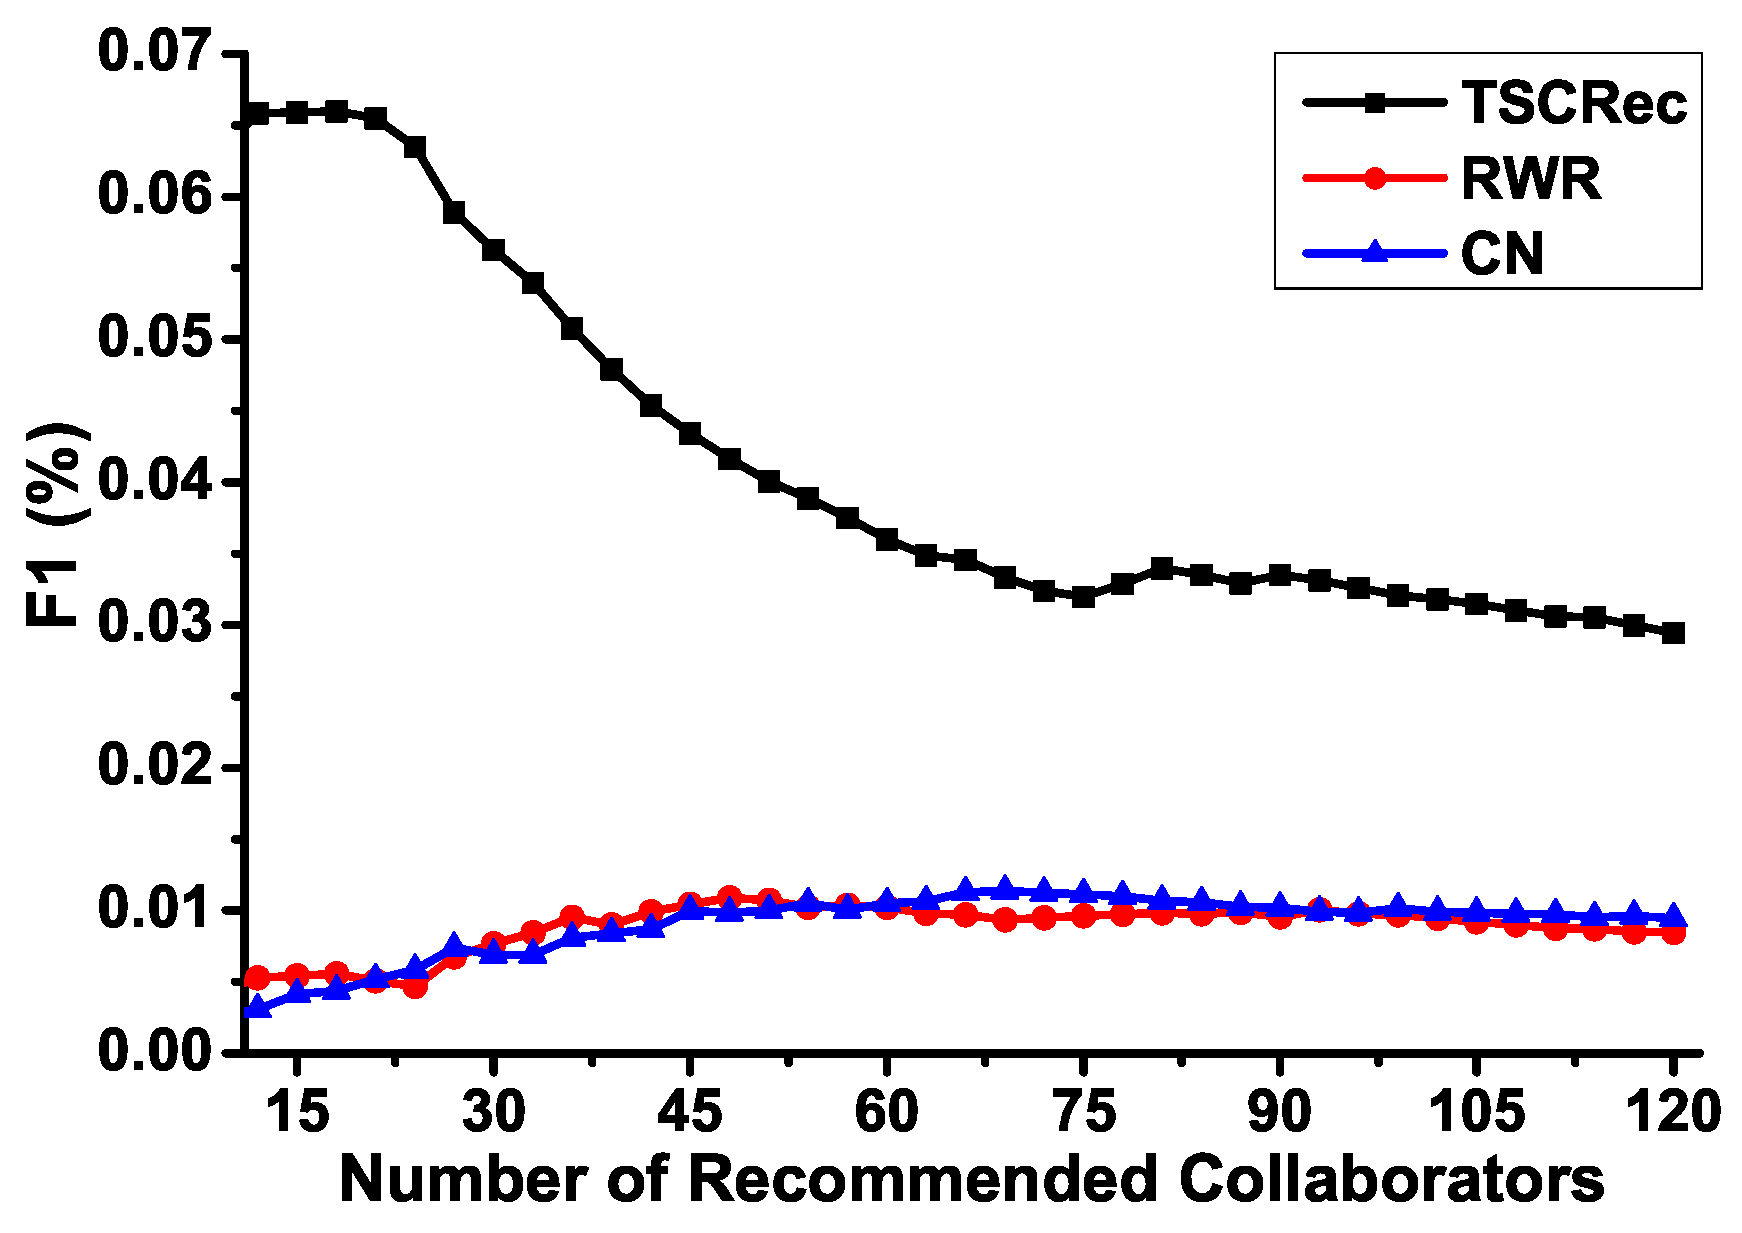
\includegraphics[width=0.32\textwidth]{Fig2-c.eps}}
\caption{Performance of TSCRec, RWR and FOF}
\label{fig:5}       % Give a unique label
\end{figure*}
We have conducted experiments with data sets of all Data Mining on DBLP. We take the year 2011 as the partition of training set and testing set. To better evaluate our model, we compared CCRec with two traditional approaches Random Walk with Restart (RWR) [1] and Common Neighbors (CN) [2]. And the metrics to evaluate the performance are precision, recall rate and F1. What we should illustrate is that we just recommend the new collaborators who never cooperated with the scholar, because the new collaborators are more meaningful and practical in real academic filed.

Figures above show the performance comparison of CCRec, RWR and CN in precision, recall rate and F1. From the experimental results, it can be observed that CCRec significantly outperforms RWR and CN. Figure 1 reveals that the precision of CCRec is always higher than that of RWR and CN. It shows an upward tendency for the recall rate of CCRec, which is obviously superior to RWR and CN. For the F1, CCRec exceeds RWR and CN all the time, and it reaches the peak 6.598\% when recommending 18 scholars.

In short, CCRec outperforms RWR and CN with higher precision, recall rate and F1. This is because CCRec with content of publications and collaboration network combined has a distinct advantage in recommending new collaborators.

% =============================================================================
\section{Concluding Remarks}
% =============================================================================
The conclusions we reach are: 1) CCRec outperforms RWR and CN in precision, recall rate and F1 integrating the content of publications with academic collaboration network. 2) With topic clustering, the problem of topic drift has been well solved.

Our research on CCRec reveals the combination of research field and his academic collaboration network can not be ignored when recommending collaborators. With the two taken into account, the results of collaborators recommendation are more specific and effective. While we need to explore more on how to enhance the performance better and take more comparison experiments.


\balance
\bibliographystyle{acm-sigchi}
\bibliography{sample}

\end{document}
